\documentclass{article}
\usepackage{pgf,tikz,tikzscale} 
\usepackage{amssymb}
\usepackage{tcolorbox}
\usepackage{tkz-berge}
\usepackage{xcolor}
\usepackage[utf8]{inputenc}
\usepackage[english]{babel}
\usepackage{multicol}
\usepackage{enumerate}	
\usepackage{graphicx,lipsum,pgfplots} 
\usepackage{amsmath, amsthm}                 
\usepackage[top=1in,bottom=1in, left=1in, right=1in] {geometry}  
\usepackage{fancyhdr}       
\usepackage{blkarray}

\tikzstyle{peers}=[draw,circle,violet,bottom color=\lav,
                  top color= white, text=violet,minimum width=10pt]


\pagestyle{fancy}              
\lhead{Math 5563 \newline Graph Theory HW7, Ch5}   
\rhead{Warren Keil}







\begin{document}
\setlength{\parindent}{0cm}   %%%%%%%% KEEP THIS  for block style paragraphs. 



%\textbf{11a.}  Suppose \(G\) is a graph on \(n\leq5\) vertices such that \(G\) is not coplanar. Prove that \(G=K_5\) or \(G=K_5^c\). 


%\vspace{3mm}
%\textit{Proof.} Let \(G\) be a graph on \(n\leq5\) vertices such that \(G\) is not coplanar. 

\textbf{1a.} Determine whether \(G\) is hamiltonian and justify your answer. 


\vspace{3mm}
\textit{Solution.}  Recall that Theorem 5.2 shows us that \textit{every hamiltonian graph is 2-connected}. We then observe what happens if we remove the following single vertex from the graph:


\begin{center}
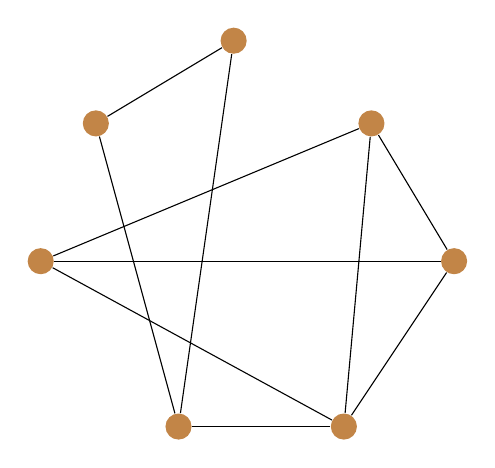
\begin{tikzpicture}
  [scale=.35,auto=left,every node/.style={circle,fill=brown!96}]
  \node (a) at (0,0) {};
  \node (b) at (6,0)  {};
  \node (c) at (10,6)  {};
  \node (d) at (7,11)  {};
  \node (e) at (2,14)  {};
  \node (f) at (-3,11)  {};
  \node (g) at (-5,6)  {};
  
  \foreach \from/\to in {a/b, b/c, c/d, e/f, a/f, a/e, g/b,g/c,g/d,b/d}
    \draw (\from) -- (\to);

\end{tikzpicture}\hspace{2cm}
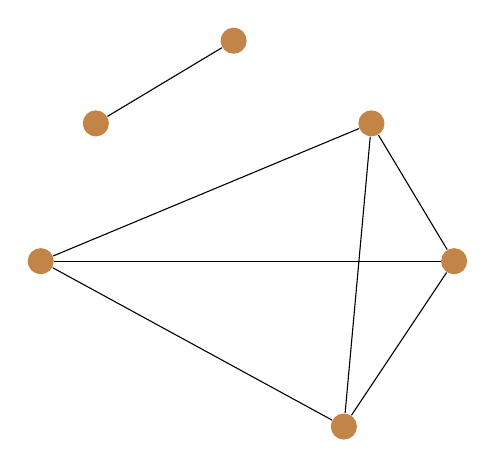
\begin{tikzpicture}
  [scale=.35,auto=left,every node/.style={circle,fill=brown!96}]
  %\node (a) at (0,0) {};
  \node (b) at (6,0)  {};
  \node (c) at (10,6)  {};
  \node (d) at (7,11)  {};
  \node (e) at (2,14)  {};
  \node (f) at (-3,11)  {};
  \node (g) at (-5,6)  {};
  
  \foreach \from/\to in { b/c, c/d, e/f, g/b, g/c, g/d, b/d}
    \draw (\from) -- (\to);
\end{tikzpicture}
\end{center}
Thus since we showed that the removal of a single vertex resulted in an increase in the number components of \(G\) then \(G\) is not 2-connected. \(\therefore G\) cannot be hamiltonian. 




\vspace{6mm}

\textbf{2.} Show that the conclusion of Ore's Lemma does not follow from the weaker hypothesis \(d(u)+d(v) \geq n-1\). 

\vspace{3mm}
\textit{Solution.} To show that Ore's Lemma does not hold for the weaker hypothesis, \(d(u)+d(v) \geq n-1\), consider the two graphs below called \(G\) and \(G_1\) respectively.

\begin{center}
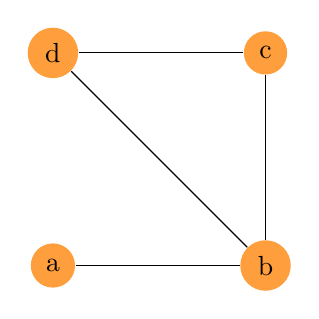
\begin{tikzpicture}
  [scale=.45,auto=left,every node/.style={circle,fill=orange!76}]
  \node (a) at (0,0) {a};
  \node (b) at (6,0)  {b};
  \node (c) at (6,6)  {c};
  \node (d) at (0,6)  {d};
  
  \foreach \from/\to in { a/b, b/c, c/d, b/d}
    \draw (\from) -- (\to);
\end{tikzpicture}\hspace{20mm}
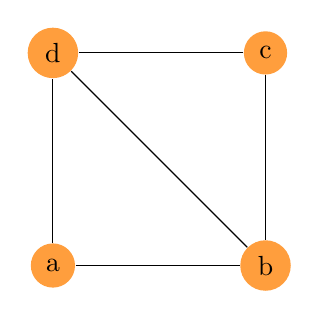
\begin{tikzpicture}
  [scale=.45,auto=left,every node/.style={circle,fill=orange!76}]
  \node (a) at (0,0) {a};
  \node (b) at (6,0)  {b};
  \node (c) at (6,6)  {c};
  \node (d) at (0,6)  {d};
  
  \foreach \from/\to in { a/b, b/c, c/d, b/d, a/d}
    \draw (\from) -- (\to);
\end{tikzpicture}
\end{center}

We see that \(n=4\) for these graphs. Also notice that the degree of vertex \(d\) in \(G\) is 2 and the degree of vertex \(a\) in \(G\) is 1. So \( d(d) + d(a) \geq 4-1 = 3 \). Thus we obtain the graph on the right \(G_1\) by adding the edge \(ad\). And clearly, \(G_1\) is hamiltonian but \(G\) is not. Thus, Ore's Lemma does not hold for the weaker hypothesis, \(d(u)+d(v) \geq n-1\).


\newpage
\textbf{4a.} Show that \(K_{3,4}\) does not have any hamiltonian cycles. 

\vspace{4mm} 

\textit{Solution.} To show that \(K_{3,4}\) does not have any hamiltonian cycles, recall theorem 5.3 which states, \textit{ if G is hamiltonian, and S is a vertex cut, then the number of components of G-S is at most the cardinality of S.} Using the contrapositive of this theorem, let \(S\) be the vertex cut consisting of the vertices \(\{g,f,e\}\). Then the number of components, \(\xi(G-S) = 4\) and the cardinality of \(S\) is 3. Thus by theorem 5.3, \(K_{3,4}\) cannot be hamiltonian. 


\begin{center}
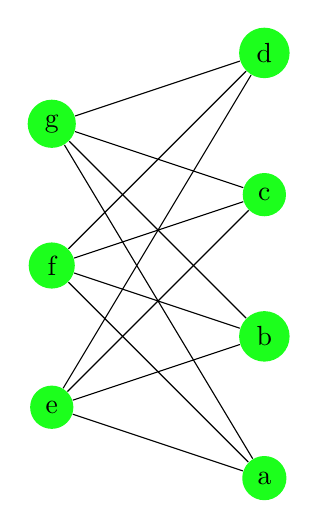
\begin{tikzpicture}
  [scale=.45,auto=left,every node/.style={circle,fill=green!89}]
  \node (a) at (6,0) {a};
  \node (b) at (6,4)  {b};
  \node (c) at (6,8)  {c};
  \node (d) at (6,12)  {d};
  \node (e) at (0,2)  {e};
  \node (f) at (0,6)  {f};
  \node (g) at (0,10)  {g};
  
  \foreach \from/\to in {g/d,g/c,g/b,g/a,f/d,f/c,f/b,f/a,e/d,e/c,e/b,e/a}
    \draw (\from) -- (\to);
\end{tikzpicture}



\end{center}


\vspace{6mm}

\textbf{18a.} Show that \(C_4\) is hamiltonian but not hamiltonian connected. 

\vspace{3mm}
\textit{Solution.} The definition of a hamiltonian cycle of a graph is a cycle that contains every vertex of the graph. A graph is called hamiltonian if it contains a hamiltonian cycle. So it follows that the graph, \(C_4\) clearly contains a cycle that has every vertex of itself in it. Thus \(C_4\) is hamiltonian. A \emph{hamiltonian path} is a path that contains every vertex of the graph. A graph is \emph{hamiltonian connected} if there exists a hamiltonian path from every two vertices in the graph. To show that \(C_4\) is not hamiltonian, consider the graph of \(C_4\) drawn below. Consider the vertices \(A\) and \(C\). The only two paths that exist between \(A\) and \(C\) are \( [A,D,C]\), \([A,B,C]\), \([C,B,A]\), and \([C,D,A]\). Since none of these paths are hamiltonian paths then \(C_4\) is not hamiltonian connected.  \(\qed\)

\begin{center}
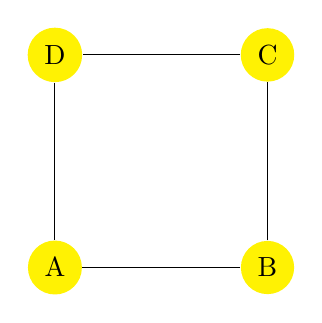
\begin{tikzpicture}
  [scale=.45,auto=left,every node/.style={circle,fill=yellow!99}]
  \node (a) at (0,0) {A};
  \node (b) at (6,0)  {B};
  \node (c) at (6,6)  {C};
  \node (d) at (0,6)  {D};
  \foreach \from/\to in {a/b,b/c,c/d,d/a}
    \draw (\from) -- (\to);
\end{tikzpicture}
\end{center}








\end{document}
